\documentclass[12pt]{article}
\usepackage[margin=2cm]{geometry}
\usepackage{amsmath}
\usepackage{slashed}
\usepackage{tikz}

\begin{document}

\noindent
Consider an electron scattered by an atomic nucleus.
\begin{center}
\begin{tikzpicture}
\draw[dashed] (0,0) circle (0.5cm);
%\draw[dashed] (1.4,0) -- (0.6,0);
\draw[thick,->] (-2,0) node[anchor=east] {$e^-$} -- (-0.6,0);
\draw[thick,->] (0.40,0.40) -- (1.3,1.3) node[anchor=south west] {$e^-$};
\draw (1,0.5) node {$\theta$};
\end{tikzpicture}
\end{center}

\noindent
Here is the same diagram with momentum and spinor labels.
\begin{center}
\begin{tikzpicture}
\draw[dashed] (0,0) circle (0.5cm);
%\draw[dashed] (1.4,0) -- (0.6,0);
\draw[thick,->] (-2,0) node[anchor=east] {$p_1,u_1$} -- (-0.6,0);
\draw[thick,->] (0.40,0.40) -- (1.3,1.3) node[anchor=south west] {$p_2,u_2$};
\draw (1,0.5) node {$\theta$};
\end{tikzpicture}
\end{center}

\noindent
The path of the incident electron can be modeled as the $z$ axis,
resulting in the following momentum vectors.
\begin{equation*}
\underset{\text{inbound electron}}
{p_1=\begin{pmatrix}E\\0\\0\\p\end{pmatrix}}
\qquad
\underset{\text{outbound electron}}
{
p_2=\begin{pmatrix}
E\\
p\sin\theta\cos\phi\\
p\sin\theta\sin\phi\\
p\cos\theta
\end{pmatrix}
}
\end{equation*}

\noindent
Symbol $p$ is electron momentum,
$E$ is total energy $E=\sqrt{p^2+m^2}$,
and $m$ is electron mass.
Polar angle $\theta$ is the observed scattering angle.
Azimuth angle $\phi$ cancels out in scattering calculations.

\bigskip
\noindent
The spinors are
\begin{equation*}
\underset{\text{inbound electron, spin up}}
{u_{11}=\begin{pmatrix}E+m\\0\\p\\0\end{pmatrix}}
\qquad
\underset{\text{inbound electron, spin down}}
{u_{12}=\begin{pmatrix}0\\E+m\\0\\-p\end{pmatrix}}
\qquad
\underset{\text{outbound electron, spin up}}
{u_{21}=\begin{pmatrix}E+m\\0\\p_{2z}\\p_{2x}+ip_{2y}\end{pmatrix}}
\qquad
\underset{\text{outbound electron, spin down}}
{u_{22}=\begin{pmatrix}0\\E+m\\p_{2x}-ip_{2y}\\-p_{2z}\end{pmatrix}}
\end{equation*}

\noindent
The spinors shown above are not individually normalized.
Instead, a combined spinor normalization constant $N=(E+m)^2$ will be used.

\bigskip
\noindent
The following formula computes a probability density $|\mathcal{M}_{ab}|^2$ for Rutherford scattering
where $a$ is the spin state of the inbound electron and $b$ is the spin state of the outbound electron.
\begin{equation*}
|\mathcal{M}_{ab}|^2=\frac{Z^2e^4}{q^4}\frac{1}{N}\left|\bar{u}_{2b}\gamma^0 u_{1a}\right|^2
\end{equation*}

\noindent
Symbol $Z$ is the atomic number of the nucleus,
$e$ is electron charge,
and $q=p_1-p_2$ is momentum transfer.

\bigskip
\noindent
The expected probability density
$\langle\vert\mathcal{M}\vert^2\rangle$
is computed by summing $|\mathcal{M}_{ab}|^2$
over all four spin states and then dividing by the number of inbound states.
There are two inbound states.
\begin{align*}
\langle\vert\mathcal{M}\vert^2\rangle
&=\frac{1}{2}\sum_{a=1}^2\sum_{b=1}^2\left|\mathcal{M}_{ab}\right|^2
\\
&=\frac{Z^2e^4}{2q^4}\frac{1}{N}\sum_{a=1}^2\sum_{b=1}^2\left|\bar{u}_{2b}\gamma^0 u_{1a}\right|^2
\\
&=\frac{Z^2e^4}{2q^4}\mathop{\rm Tr}\left((\slashed{p}_1+m)\gamma^0(\slashed{p}_2+m)\gamma^0\right)
\\
&=\frac{2Z^2e^4}{q^4}\left(E^2+m^2+p^2\cos\theta\right)
\end{align*}

\noindent
Run ``rutherford-scattering-1.txt'' to verify the following formulas.
\begin{gather*}
\frac{1}{N}\sum_{a=1}^2\sum_{b=1}^2\left|\bar{u}_{2b}\gamma^0 u_{1a}\right|^2
=\mathop{\rm Tr}\left((\slashed{p}_1+m)\gamma^0(\slashed{p}_2+m)\gamma^0\right)
=4(E^2+m^2+p^2\cos\theta)
\\
q^4=(p_1-p_2)^4=16p^4\sin^4(\theta/2)=4p^4(\cos\theta-1)^2
\end{gather*}

\subsection*{Low energy approximation}
For low energy electrons such that $p\ll m$ we can use the following approximation.
\begin{equation*}
E^2+m^2+p^2\cos\theta\approx2m^2
\end{equation*}

\noindent
Hence
\begin{equation*}
\langle|\mathcal{M}|^2\rangle=\frac{4m^2Z^2e^4}{q^4}
\end{equation*}

\noindent
Substituting $e^4=16\pi^2\alpha^2$ and $q^4=4p^4(\cos\theta-1)^2$ we have
\begin{equation*}
\langle|\mathcal{M}|^2\rangle=\frac{16\pi^2m^2Z^2\alpha^2}{p^4(\cos\theta-1)^2}
\end{equation*}

\noindent
The differential cross section is
\begin{equation*}
\frac{d\sigma}{d\Omega}=\frac{\langle|\mathcal{M}|^2\rangle}{16\pi^2}
=\frac{m^2Z^2\alpha^2}{p^4(\cos\theta-1)^2}
\end{equation*}

\noindent
We can integrate $d\sigma$ to obtain a cumulative distribution function.
Recall that
\begin{equation*}
d\Omega=\sin\theta\,d\theta\,d\phi
\end{equation*}
Hence
\begin{equation*}
d\sigma=\frac{m^2Z^2\alpha^2}{p^4(\cos\theta-1)^2}\sin\theta\,d\theta\,d\phi
\end{equation*}

\noindent
Let $I(\theta)$ be the following integral of $d\sigma$.
\begin{align*}
I(\theta)
&=\left(\frac{p^4}{m^2Z^2\alpha^2}\right)\frac{1}{2\pi}\int_0^{2\pi}\int d\sigma
\\
&=\int\frac{1}{(\cos\theta-1)^2}\sin\theta\,d\theta
\\
&=\frac{1}{\cos\theta-1},\quad a\le\theta\le\pi
\end{align*}

\noindent
Angular support is limited to an arbitrary $a>0$ because $I(0)$ is undefined.

\bigskip
\noindent
Let $C$ be the normalization constant
\begin{equation*}
C=I(\pi)-I(a)
\end{equation*}

\noindent
Then the cumulative distribution function $F(\theta)$ is
\begin{equation*}
F(\theta)=\frac{I(\theta)-I(a)}{C},
\quad a\le\theta\le\pi
\end{equation*}

\noindent
The probability of observing scattering events
in the interval $\theta_1$ to $\theta_2$ can now be computed.
\begin{equation*}
P(\theta_1\le\theta\le\theta_2)=F(\theta_2)-F(\theta_1)
\end{equation*}

\noindent
Probability density function $f(\theta)$ is the derivative of $F(\theta)$.
\begin{equation*}
f(\theta)=\frac{dF(\theta)}{d\theta}
=\frac{\sin\theta}{C(\cos\theta-1)^2}
\end{equation*}

\noindent
Run ``rutherford-scattering-3.txt'' to draw a graph of $f(\theta)$ for $a=\pi/4=45^\circ$.

\begin{center}
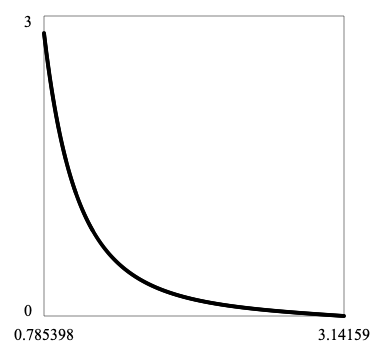
\includegraphics[scale=0.5]{rutherford-scattering-1.png}
\end{center}

\noindent
Probability distribution for $45^\circ$ bins ($a=45^\circ$).

\begin{center}
\begin{tabular}{|c|c|c|}
\hline
$\theta_1$ & $\theta_2$ & $P(\theta_1\le\theta\le\theta_2)$\\
\hline
$0^\circ$ & $45^\circ$ & -- \\
$45^\circ$ & $90^\circ$ & 0.83 \\
$90^\circ$ & $135^\circ$ & 0.14 \\
$135^\circ$ & $180^\circ$ & 0.03 \\
\hline
\end{tabular}
\end{center}

\bigskip
\noindent
Note:
The original Rutherford scattering experiment in 1911 used alpha particles, not electrons.
However, scattering of any charged particle by Coulomb interaction
is now known as Rutherford scattering.
The first Rutherford scattering experiment using electrons appears to have
been done by F.~L.~Arnot, then a student of Rutherford, in 1929.

\end{document}
